\documentclass[12pt]{galois-whitepaper}
\usepackage{listings}
\usepackage{float}
\usepackage{xspace}
\usepackage{color}
\usepackage{tikz}
\usepackage{url}
\usepackage{amsmath}
\usepackage{amsfonts}
\usepackage{amssymb}
\usepackage{amscd}
\usepackage{verbatim}
\usepackage{subcaption}
\usepackage{fancyvrb}
\usepackage{multirow}
\let\verbatiminput=\verbatimtabinput
\VerbatimFootnotes
\DefineVerbatimEnvironment{code}{Verbatim}{}
\DefineVerbatimEnvironment{pseudoCode}{Verbatim}{}
%\hyphenation{Saw-Script}
%\newcommand{\sawScript}{{\sc SawScript}\xspace}

\usepackage[all,2cell]{xy}
\UseAllTwocells

\usepackage{textcomp}

\renewcommand{\textfraction}{0.05}
\renewcommand{\topfraction}{0.95}
\renewcommand{\bottomfraction}{0.95}
\renewcommand{\floatpagefraction}{0.35}
\setcounter{totalnumber}{5}
\definecolor{MyGray}{rgb}{0.9,0.9,0.9}
\makeatletter\newenvironment{graybox}{%
   \begin{lrbox}{\@tempboxa}\begin{minipage}{\columnwidth}}{\end{minipage}\end{lrbox}%
   \colorbox{MyGray}{\usebox{\@tempboxa}}
}\makeatother

\setlength{\parskip}{0.6em}
\setlength{\abovecaptionskip}{0.5em}

\lstset{
         basicstyle=\footnotesize\ttfamily, % Standardschrift
         %numbers=left,               % Ort der Zeilennummern
         numberstyle=\tiny,          % Stil der Zeilennummern
         %stepnumber=2,               % Abstand zwischen den Zeilennummern
         numbersep=5pt,              % Abstand der Nummern zum Text
         tabsize=2,                  % Groesse von Tabs
         extendedchars=true,         %
         breaklines=true,            % Zeilen werden Umgebrochen
         keywordstyle=\color{red},
                frame=lrtb,         % left, right, top, bottom frames.
 %        keywordstyle=[1]\textbf,    % Stil der Keywords
 %        keywordstyle=[2]\textbf,    %
 %        keywordstyle=[3]\textbf,    %
 %        keywordstyle=[4]\textbf,   \sqrt{\sqrt{}} %
         stringstyle=\color{white}\ttfamily, % Farbe der String
         showspaces=false,           % Leerzeichen anzeigen ?
         showtabs=false,             % Tabs anzeigen ?
         xleftmargin=10pt, % was 17
         xrightmargin=5pt,
         framexleftmargin=5pt, % was 17
         framexrightmargin=-1pt, % was 5pt
         framexbottommargin=4pt,
         %backgroundcolor=\color{lightgray},
         showstringspaces=false      % Leerzeichen in Strings anzeigen ?
}

\author{Eric Davis, Alec Theriault, and Ryan Wright}
\title{AMIDOL Milestone 13 and 14 Report}
\date{1/30/2020}
\begin{document}
\maketitle

\vspace*{2cm}
\tableofcontents

\section{Introduction}

\begin{figure}
  \centering
  \includegraphics[width=0.5\textwidth]{figs/AMIDOL-architecture.png}
  \caption{AMIDOL Architecture}
  \label{Fig:Arch}
\end{figure}

\part{Milestone 13}

\section{Recent Extensions to the AMIDOL Framework}

The UI for comparing results of multiple models has been extended to support a rich language for combining traces. This is particularly useful for constructing derived measures without needing to re-run the model. For instance, this might be used in a situation where an epidemiological model tracks multiple strains of a virus separately, but the hospital data only keeps aggregate data. Another similar case is when the scientist doing modelling is trying to quickly line up peaks of infected populations from model result and real world data. Our language contains primitives like shift which simplify this sort of transformation.

A completely new VDSOL that is designed to take a system of
differential equations written in LaTeX format has been added. The
idea behind this new language is to simplify the work of going from a
model written in an academic paper to an AMIDOL model. Scientists
enter LaTeX equations, constants, and initial conditions in a text
box. Beside this input, they get a real-time LaTeX preview of their
equations. From there, the model is compiled into the AMIDOL IR so
that it can be executed and compared to results from other models
(which may have been designed in completely different VDSOLs).

Finally, we are in the process of experimenting with model composition in the backend, with the goal of finding a minimal intuitive language for combining models. To this end, we’ve been refining our existing state-sharing composition operators and have started to experiment with other techniques revolving around substitution. Most of these changes are still not exposed to end users, since we are not yet sure what a good visual representation would look like.

\subsection{VDSOLs for Mathematical Languages}

Adding a VDSOL for LaTeX input equations: The VDSOL renders LaTeX
equations using KaTeX, a fast browser-based Javascript library
designed for this purpose. Once a user submits a system of
differential equations, the backend tries to parse each line as a
differential equation, initial condition, or constant. This step is
complicated by the fact that the LaTeX source for equations can
sometimes be interpreted in multiple ways (for instance: is
`\textbackslash frac{psi}{2}` the variable `psi` divided by two, or the product of `p`, `s`, `i`, and `0.5`). To solve this ambiguity, we require that implied multiplication include at least a space to separate the factors (eg. `p s i` vs `psi`). The final step is to convert the system of differential equations into an AMIDOL model. This is fairly straightforward: variables in the equations turn into states and the right-hand side of the equations turns into events.

\subsection{Definition of Derived Measures}

Updating the comparison UI to support a richer mathematical language for derived measures:  In order to implement this, we’ve moved the work of combining data traces from the UI to the backend. The language for describing derived measures supports translations, linear distortions, component-wise arithmetic, as well as a couple built-in math functions. The backend contains a parser for this language as well as an interpreter. One of the challenges here is around how to interpolate when combing data traces whose measures had different time ranges or step sizes.

\section{AMIDOL Demo Instructions}

\begin{figure}
  \centering
  \includegraphics[width=0.5\textwidth]{figs/LaTex_VDSOL_results.png}
  \caption{AMIDOL Architecture}
  \label{Fig:Arch}
\end{figure}

\begin{figure}
  \centering
  \includegraphics[width=0.5\textwidth]{figs/LaTeX_VDSOL.png}
  \caption{AMIDOL Architecture}
  \label{Fig:Arch}
\end{figure}

\begin{figure}
  \centering
  \includegraphics[width=0.5\textwidth]{figs/SIIR_setup_comparision.png}
  \caption{AMIDOL Architecture}
  \label{Fig:Arch}
\end{figure}

\begin{figure}
  \centering
  \includegraphics[width=0.5\textwidth]{figs/SIIR_visualize_comparision.png}
  \caption{AMIDOL Architecture}
  \label{Fig:Arch}
\end{figure}

\begin{figure}
  \centering
  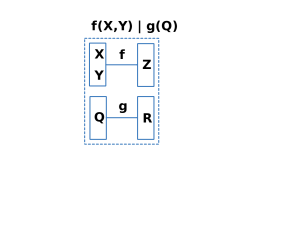
\includegraphics[width=0.5\textwidth]{figs/parallel.png}
  \caption{AMIDOL Architecture}
  \label{Fig:Arch}
\end{figure}

\begin{figure}
  \centering
  \includegraphics[width=0.5\textwidth]{figs/serial.png}
  \caption{AMIDOL Architecture}
  \label{Fig:Arch}
\end{figure}

\begin{figure}
  \centering
  \includegraphics[width=0.5\textwidth]{figs/substitution.png}
  \caption{AMIDOL Architecture}
  \label{Fig:Arch}
\end{figure}

\section{AMIDOL Performance for Real-World Systems and Processes}

{ \footnotesize
\begin{tabular}{|llllll|}
 \hline
  & \textbf{Model}	& \textbf{SIR}	& \textbf{SIIR}	& \textbf{Predator-Prey}	&
                                                  \textbf{SIR with}\\
  & & & & & \textbf{vital dynamics}\\
  \hline
   \multirow{6}{*}{\textit{Time}}     & Graph VDSOL to IR compilation	& 1.7ms	& 1.7ms	& 1.1ms	&
                                                                  1.6ms\\
  & Julia to Graph VDSOL
                & 1.8s - 6s	&2.1s - 6s	& n / a	& n / a\\
  & (including ontology grounding search) & & & &\\
        & IR compilation to Python backend	& 190ms	& 160ms & 30ms
                                                                  &
                                                                    160ms\\
        & IR compilation to Julia backend & 24ms	& 25ms	& 15ms
                                                & 52ms\\
        & Execution of Python backend output	& 2.5s	& 2.4s	& 1.1s
                                                & 2.5s\\
	& Execution of Julia backend output	& 9.8s	& 12s	& 7.5s
                                                & 7.0s\\
  \hline
  \hline
  \multirow{2}{*}{\textit{Lines of Code}} & Python backend output & 40
                                        & 45 & 39	& 47\\
        & Julia backend output	& 44	& 62	& 51	& 60\\
  \hline
\end{tabular}
}

\part{Milestone 14}

\section{Final Prototype Development}

\section{AMIDOL as a Service}

\begin{figure}
  \centering
  \includegraphics[width=0.5\textwidth]{figs/AMIDOL-service.png}
  \caption{AMIDOL as a Service}
  \label{Fig:Service}
\end{figure}

\subsection{Read/Write Model}

Summary – Allow external applications to read and write models to AMIDOL’s IR.

Requirements – Working to supplement AMIDOL with searchable model database, supporting a query interface for model properties and UUIDs for models.

\subsection{Infer/Read VDSOL}

Summary – Currently supports VDSOL inference from AMIDOL IR or Julia code with groundings.

Requirements – Allows retrieval of VDSOLs by UUID and query interface for VDSOL properties.

\subsection{Read/Write Results}

Summary – Allow external applications to read and write to the AMIDOL results database.

Requirements – AMIDOL is implementing a graph-based results database,
including mechanisms to index into the database to write external
results (from “data” or an “external model”).

Suggestions – Measure indexing by outside applications is an open question.  We need a clear definition of measure equivalence.  What does it mean for two measures to be the same?  At a basic level, they have the same sigma-algebraic structure, over borel sets that are proxies for the same space.  What does this mean in practice?

\subsection{Transform/Execute Model}

Summary – Allow external applications transform a model in AMIDOL, and to execute a model in AMIDOL.

Requirements – Valid transformation set.  This is essentially a model transformation algebra.

\section{Model Algebras and Transformations}

Models form a group with the operation ”.” (serial composition).
Closed
Associative
Identity element
The “pass through” model which immediately yields its inputs without changing them.
Inverse element is a bit harder.
Intuitively you need a model which ”undoes” g() yielding no output, and passes through the inputs to f().



\subsection{Composing Models in AMIDOL}

Composition via state sharing is very powerful: we’ve built prototypes that combine birth-death processes, the SIRS model, Lokta-Volterra predator prey, and population flow models. Some of the challenges we’ve identified in this space:

Naming shared states, especially when multiple states are being combined. The most promising avenue is to find a way to force users to specify names.

It should be possible to provide some automated assistance about which compositions make sense or don’t based on units / types / ontological categories

Sub-models being composed need to be pretty general to account for different ways in which we may want to specialize them through composition. One idea to help deal with this is using substitution to introduce new states into existing models.

\subsection{Substituting Models in AMIDOL}

Substitution of subgraphs (of events and states) with other compatible subgraphs
Provides a mechanism for quickly swapping out sub-models used in a bigger model (for instance: changing an SIR model into an SEIR one).
Required inputs: the states to remove, the events (between these states) to remove, the new model to introduce, and a mapping from the removed states to the states in the new model.
Challenge: it is possible for subgraph substitution to accidentally “break” some other part of the model. Consider the case of swapping an SIR sub-model for an SEIR sub-model: elsewhere in the larger model, uses of $S + I + R$ probably indicated “total population” and should be replaced with $S + I + E + R$.
Solution idea: provide a mechanism for building up symbolic expressions $total_{population} = S + I + R$ that can be used multiple times in the bigger model. This alleviates the pain of “refactoring” after substitution.
Solution idea: bring to the users attention all locations in the model where there are references to state variables that are part of substitution
Challenge: sometimes, we want to be able to do multiple substitutions
in parallel. For instance, we want to replace every instance of a
sub-model with some other sub-model. In this case, model substitution
turns into what looks like a structural graph query problem.

One useful take of substitution involves introducing new states into existing models. For instance: a rate in a model starts by being approximated using a constant but eventually needs to be turned into a proper state (the model is being run with parameters where the constant assumption no longer holds - think a pendulum that goes from small-angle swings to large-angle ones).
Challenge: this sort of transformation seems painfully low-level - is there some bigger operations that generalizes this nicely?

\end{document}